\documentclass[12pt,a4paper]{article}
\usepackage[a4paper,top=1.5cm, bottom=1.5cm, left=1.5cm, right=1.5cm]{geometry}
\usepackage[T2A]{fontenc}
\usepackage[utf8]{inputenc}
\usepackage[russian]{babel}
\usepackage{amsmath}
\usepackage{amssymb}
\usepackage{hyperref}
\usepackage{graphicx}
\usepackage{floatrow}
\usepackage{booktabs}
\usepackage{wrapfig}
\usepackage{indentfirst}
\usepackage{lipsum}
\usepackage{subcaption}
\usepackage{float}
%\usepackage{derivative}
\usepackage{enumitem}
\restylefloat{table}

\newcommand{\figref}[1]{(см. рис. \ref{#1})}
\newcommand{\e}[1]{\text{$\cdot10^{#1}$}}

\title{Лабораторная работа 3.4.1\\ Исследование диа- и парамагнетиков}
\author{Симанкович Александр \\ Маслов Артём \\ Б01-104}
\date{30.09.2022}

\begin{document}
	\maketitle
	
	\section*{Аннотация}
	
	В работе приводится эмпирическая теория диамагнетиков и парамагнетиков. Измеряется магнитная восприимчивость образцов меди, алюминия, графита и вольфрама.
		
	\vspace{10pt}
	\noindent\textbf{Ключевые слова}: диамагнетики, парамагнетики.
	
	\section*{Введение}
	
	Из опытов известно, что вещество может реагировать на внешнее магнитное поле. Из-за внутренней структуры парамагнетики (<<усиливают>>) и диамагнетики (<<ослабляют>>) довольно слабо меняют результирующее поле: изменение поля составляет $10^{-4} \div 10^{-8}$ от внешнего. Ферромагнетики, напротив, усиливают внешнее магнитное поле в $10^3 \div 10^4$ раз.
	
	Согласно уравнениям Максвелла, магнитное поле создаётся движущимися зарядами. Магнитное поле также создаётся орбитальным движением электронов вокруг атомов и собственным вращением электронов (спином) и ядер. Полноценное описание магнитных свойств вещества возможно только при применении квантовой механики. В данной работе приводится полуклассическая модель магнитного поля в веществе. Предполагается, что электроны и ядра не обладают собственным вращением.
			
	Данная работа была проведена в рамках учебного исследовательского курса в Московском физико-техническом институте. Целью работы является подтверждение теории, описывающей взаимодействия диа- и парамагнетиков с магнитным полем, и определение магнитной восприимчивости меди, алюминия, графита и вольфрама.
	
	\section*{Теоретическое введение}
	\subsection*{Эмпирическая теория магнитных свойств вещества}
	
	Магнитное поле на уровне атомов может резко изменяться в пространстве и времени. Такую физическую величину практически невозможно измерить, поэтому рассматриваются физически бесконечно малые объёмы вещества. Такой объём вещества достаточно мал, чтобы его размерами можно было пренебречь, но содержит достаточно большое количество частиц, чтобы магнитное микрополе можно было усреднить.
	
	Для описания усредненного магнитного поля вводится вектор \textit{намагниченности} $\boldsymbol{M}$, который равен суммарному магнитному дипольному моменту единицы объёма. Тогда средняя индукция магнитного поля в данном бесконечно малом объёме равна:
	$$
	\boldsymbol{B} = \mu_0 (\boldsymbol{H} + \boldsymbol{M}),
	$$
	$\mu_0 = 4 \pi \cdot 10^{-7}$ -- магнитная постоянная.
	
	В простейшем случае намагниченность сонаправлена с вектором напряженности внешнего магнитного поля:
	$$
	\boldsymbol{M} = \chi \boldsymbol{H}
	$$
	Коэффициент $\chi$ называется магнитной восприимчивостью среды.

	Тогда индукция магнитного поля равна:
	$$
	\boldsymbol{B} =  \mu_0 (1 + \chi) \boldsymbol{H} = \mu_0 \mu \boldsymbol{H}
	$$
	
	Данная модель достаточно груба, по следующим соображениям:
	\begin{enumerate}
		\item $\boldsymbol{M}$ может быть не сонаправлена с $\boldsymbol{H}$.

		\item Зависимость $\boldsymbol{M}(\boldsymbol{H})$ может быть не линейной.
		
		\item $\boldsymbol{M}$ может зависеть от предыдущих состояниях вещества --- явление гистерезиса.
	\end{enumerate}
	Тем не менее, данная модель дает правильные по порядку результаты.
	
	Наличие внешнего магнитного поля приводит к дополнительному вращению электронов вокруг атомов так, чтобы скомпенсировать внешнее поле. При этом магнитное поле, создаваемое электронами достаточно мало. Такой механизм реакции на внешнее магнитное поле называется диамагнетизмом и он присущ всем веществам. Если диамагнетизм в веществе является основной причиной возникновения намагниченности, то такое вещество называется \textit{диамагнетиком}. Элементарные диполи в диамагнетиках в среднем ориентированы против внешнего магнитного поля, поэтому $\chi < 0$.
	
	Если энергия магнитного взаимодействия соседних атомов мала по сравнению с тепловой энергией, то магнитные моменты ориентированы хаотически. Из квантовой механики известно, что во внешнем магнитном поле магнитным моментам энергетически выгодно ориентироваться по направлению внешнего поля. Вещества, в которых элементарные диполи в основном ориентированы по направлению внешнего поля, называются \textit{парамагнетиками}.
	
	\subsection*{Магнетики в однородном магнитном поле}
	\begin{wrapfigure}{l}{0.30\textwidth}
		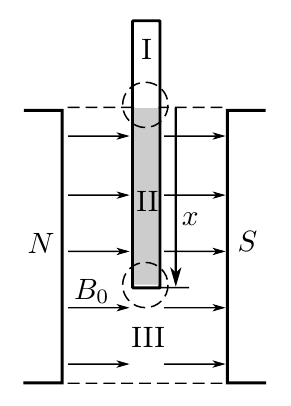
\includegraphics[width=\linewidth]{res/rod.png}
		\caption{Стержень во внешнем магнитном поле.}
		\label{img:rod}
	\end{wrapfigure}
	
	Рассмотрим тонкий, длинный стержень, помещенный во внешнее однородное магнитное поле (рис. \ref{img:rod}). Магнитное поле в данной работе создаётся электромагнитом, для того чтобы оно было однородно площадь торцов электромагнита должна быть много больше размеров стержня, и стержень должен быть помещен в середину зазора.
	
	В области $I$ магнитное поле пренебрежимо мало, в области $III$ оно примерно равно внешнему магнитному полю $B_0$. В области $II$ согласно рассматриваемой модели магнитное поле равно:
	$$
	\boldsymbol{B} = \mu \boldsymbol{H}
	$$
	На границах областей $I$ и $II$, $II$ и $III$ имеют место краевые эффекты, магнитное поле вычисляется сложно, поэтому чтобы ими можно было пренебречь стержень должен быть длинным.
	
	С помощью метода виртуальных перемещений определим силу, действующую на стержень. Пусть длина области $II$ равна $x$, стержень имеет сечение $S$.
	
	Определим поле внутри стержня. Вне стержня $B_0 = \mu_0 H_0$. Намагниченный внешним магнитным полем стержень будет вблизи создавать магнитное поле, так, что суммарное поле вблизи стержня в общем случае не будет равно внешнему магнитному полю. Для диа- и парамагнетиков $\chi \ll 1$, следовательно намагниченность стержня мала и поле вблизи него можно считать примерно равным внешнему магнитному полю. Тогда из непрерывности тангенциальной компоненты $H$ при переходе через границу находим, что напряженность внутри стержня $H_{ст} = H_0$, тогда $B_{ст} = \mu B_0$.
	
	Определим объемную плотность энергии поля в диа- и парамагнетиках. Если $\boldsymbol{B} = \mu_0 \mu \boldsymbol{H}$, то объемная энергия поля равна:
	$$
	\omega = \int{\boldsymbol{H} d\boldsymbol{B}} = \frac{B^2}{2 \mu \mu_0}
	$$
	
	Рассмотрим бесконечно малое перемещение стержня на $dx$. Объем области $II$ увеличится на $S dx$, объем области $III$ уменьшится на $- S dx$. Тогда изменение энергии магнитного поля равно:
	$$
	\Delta W = \frac{B_2^2}{2 \mu \mu_0} S dx - \frac{B_3^2}{2 \mu_0} S dx = \chi \frac{B_0^2}{2 \mu_0} S dx
	$$
	Тогда искомая сила, действующая на стержень равна:
	\begin{equation}
		F = \left( \frac{\partial W}{\partial x} \right)_{B_0} = \chi \frac{B_0^2}{2 \mu_0} S
		\label{theory:F}
	\end{equation}
	Из формулы (\ref{theory:F}) следуют, что парамагнетики втягиваются в зазор электромагнита, а диамагнетики выталкиваются.
	
	\section*{Оборудование и приборы}
	\begin{itemize}[itemsep = 0pt, parsep=0pt]
		\item Электромагнит.
		\item Аналитические весы CY-1003C. Погрешность измерения $\varsigma_m = 10^{-3}$ г.
		\item Миллитесламетр АТЕ-8702. Погрешность измерения $\varsigma_{\text{Тл}} = (0.05 \cdot B + 10) \; \text{мТл}$.
		\item Милливеберметр M119. Погрешность измерения  $\varsigma_{\text{Вб}} = (0.015 \cdot \Phi + 0.05) \; \text{мВб}$.
		\item Регулируемый источник постоянного тока GPR-11H30D. Погрешность измерения: $\varsigma_{A_1} = (0.005 \cdot I + 0.02) \; \text{А}$.
		\item Образцы меди, алюминия, графита и вольфрама.
	\end{itemize}
	
	\section*{Методика эксперимента}
	
	\begin{wrapfigure}{l}{0.5\textwidth}
		\vspace{-10pt}
		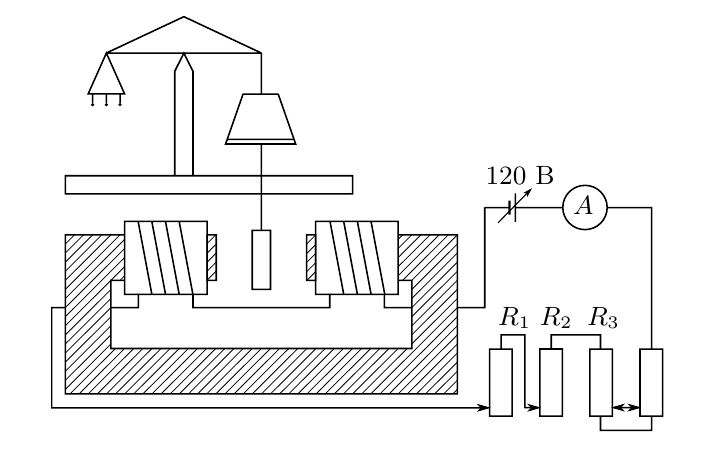
\includegraphics[width=\linewidth]{res/scheme.png}
		\caption{Схема экспериментальной установки.}
		\label{img:scheme}
	\end{wrapfigure}
		
	В данной работе для определения магнитной восприимчивости применяется \textit{метод Гюи}. Один из концов образца помещается в зазор электромагнита, другой находится в области, где магнитным полем можно пренебречь. От магнитных свойств образца зависит, будет ли он во внешнем поле втягиваться в зазор или выталкиваться из него.
	
	Схема экспериментальной установки представлена на рис. \ref{img:scheme}. Исследуемый образец подвешивают за тонкую нерастяжимую нить к чувствительному элементу аналитических весов. Показания весов обнуляют, и поэтому при дальнейших измерениях они будут показывать значение магнитной силы действующей на образец. Величину магнитного поля можно регулировать, изменяя ток через электромагнит, с помощью источника питания.
	
	Сначала проводится градуировка электромагнита. Измеряется зависимость магнитной индукции от силы тока $B(I)$. Измерения производятся милливеберметром и миллитесламетром.
	
	После этого для каждого образца измеряют зависимость действующей на образец силы от тока в электромагните $F(I)$. Измерения производятся при увеличении тока от 0 до максимального значения, а затем при уменьшении тока.
	
	Таким образом мы получаем зависимость $F(B)$, которая описывается формулой \eqref{theory:F}.
	
	\section*{Экспериментальные результаты}
	
	\subsection*{Градуировка электромагнита}
	
	На рисунке ниже приведена градуировочная кривая.
	
	\begin{figure}[H]
		\includegraphics[]{gen/electromagnet_BI.pdf}
		\caption{Зависимость поля в зазоре $B$ от протекающего тока $I$}
	\end{figure}
	
	Градуировочные графики $B(I)$ совпадают для обоих приборов в пределах погрешности. Для вычисления значения поля в последующих пунктах используется калибровка с помощью тесламетра.
	
	\subsection*{Измерение перегрузок}
	
	С помощью аналитических весов проведем измерения значения перегрузки $\Delta P$ при различных значениях поля $B$ в зазоре электромагнита. Измерения будем проводить как в прямом (\textit{рост}), так и в обратном (\textit{падение}) направлении.
	
	На рисунке ниже приведены зависимости перегрузки от квадрата индукции магнитного поля $P(B^2)$ для меди и алюминия.
	
	\begin{figure}[H]
		\includegraphics[]{gen/cu_al.pdf}
		\caption{Зависимость перегрузки $\Delta P$ от поля в зазоре $B$ для меди и алюминия}
	\end{figure}

	\begin{table}[h]
		\caption{Параметры графика $\Delta P(B^2)$ для меди}
		\input{gen/cu_mnk.tex}
	\end{table}
	
	\begin{table}[h]
		\caption{Параметры графика $\Delta P(B^2)$ для алюминия}
		\input{gen/al_mnk.tex}
	\end{table}
	
	Измеренные зависимости $\Delta P (B^2)$ являются линейными. По коэффициенту магнитной восприимчивости устанавливаем, что медь является диамагнетиком, алюминий --- парамагнетиком:
	
	$$\chi_{Cu} = -(1.08 \pm 0.03) \cdot 10^{-5} $$
	$$\chi_{Al} = +(2.17 \pm 0.03) \cdot 10^{-5} $$
	
	На рисунке ниже приведены зависимости перегрузки от квадрата индукции магнитного поля $P(B^2)$ для разных образцов графита. Один образец графита имеет дефект, это стержень, который разломили на две не одинаковые части и соединили их вместе скотчем. Такой стержень является не лучшим образцом для исследования из-за трудности описания магнитных явлений, возникающих внутри него, тем не менее для него были записаны показания. Из-за сложной структуры исследуемого образца, график является не линейным и проанализировать его невозможно. Также невозможно предложить модель, описывающую свойства такого образца в магнитном поле. Поэтому ограничимся исследованием второго образца графита, которым был цельный длинный стержень.
	
	\begin{figure}[H]
		\includegraphics[]{gen/gr.pdf}
		\caption{Зависимость перегрузки $\Delta P$ от поля в зазоре $B$ для графита}
	\end{figure}
	
	\begin{table}[h]
		\caption{Параметры графика $\Delta P(B^2)$ для целого графита}
		\input{gen/gr_mnk.tex}
	\end{table}
	
	$$\chi_{Gr} = +(2.15 \pm 0.11) \cdot 10^{-4} $$
	
	На рисунке ниже приведены зависимости перегрузки от квадрата индукции магнитного поля $P(B^2)$ для вольфрама.
	
	В качестве образцов использовались два вольфрамовых стержня. \textit{Серия 1} и \textit{серия 2} были проведены с первым и вторым образцом, соответственно. В первой и второй серии при малых полях реакции на внешнее поле не наблюдалось. Предположительно это связано с пределом точности измерений аналитических весов, поскольку максимальное значение перегрузки было $m = 12$ г. С целью уточнения результатов была проведена серия измерений со сдвоенным образцом (два образца склеили скотчем и подвесили перпендикулярно полю $B$ в зазоре электромагнита).
	
	\begin{figure}[H]
		\includegraphics[]{gen/wr_dbl.pdf}
		\caption{Зависимость перегрузки $\Delta P$ от поля в зазоре $B$ для вольфрама}
	\end{figure}
	
	\begin{table}[h]
		\caption{Параметры графика $\Delta P(B^2)$ для сдвоенного образца вольфрама}
		\input{gen/wr_dbl_mnk.tex}
	\end{table}
	
	Серия измерений для сдвоенного образца дает линейную зависимость и оценку магнитной восприимчивости $\chi_W$:
	$$\chi_{W} = +(7.24 \pm 0.26) \cdot 10^{-5} $$
	
	\section*{Выводы}
	
	В работе была измерена магнитная восприимчивость: \\
	Медь $\chi = -(1.08 \pm 0.03) \cdot 10^{-5}$. \\
	Алюминий $\chi = +(2.17 \pm 0.03) \cdot 10^{-5}$. \\
	Графит $\chi = +(21.5 \pm 1.1) \cdot 10^{-5}$. \\
	Вольфрам $\chi = +(7.24 \pm 0.26) \cdot 10^{-5}$.
	
	Табличные значения: \\
	Медь $\chi = -1.03 \cdot 10^{-5}$. \\
	Алюминий $\chi = +2.3 \cdot 10^{-5}$. \\
	Графит $\chi_\parallel = -61.0 \cdot 10^{-5}$. \\
	Графит $\chi_\perp = -14.0 \cdot 10^{-5}$. \\
	Вольфрам $\chi = +17.6 \cdot 10^{-5}$.
	
	Достаточно точно получилось измерить магнитную восприимчивость для меди и алюминия, значение $\chi$ для вольфрама удалось оценить до порядка.
	
	Результаты измерений для графита дали странное различие: табличные данные указывают, что графит является диамагнетиком, тогда как наши результаты говорят о том, что он парамагнетик. Это может объясняться тем, что в образце графита есть небольшие примеси ферромагнетика, который сильно искажает поведение образца. Другое объяснение может заключаться в том, что сам графит имеет ферромагнитные свойства из-за плоскостей точечных дефектов.\footnote{
		\href{https://www.nature.com/articles/nphys1399}{Room-temperature ferromagnetism in graphite driven by two-dimensional networks of point defects, J. Cervenka, M. I. Katsnelson and C. F. J. Flipse, 2009.}
	}.
	
\end{document}